% !TEX root = ../../Tesi.tex

%******************************************
%	Lo stage
%******************************************

\chapter{Lo stage}
\label{cap:stage}

\section{Gli stage in azienda}

Lo stage identifica un periodo lavorativo all'interno di un'azienda, svolto da una persona come se essa fosse un dipendente. L'obiettivo primario dello stage è quello di far apprendere alla persona le competenze necessarie per poter essere poi, eventualmente, assunto, divenendo così un dipendente a tutti gli effetti. \\
\nomeAzienda si adegua pienamente a questa definizione, reputando gli stage di grande interesse, con il fine di portare innovazione all'interno dell'azienda e possibilmente nuovi dipendenti. \\
Le motivazioni che spingono dunque l'azienda ad ospitare gli stage, sono molteplici:

\begin{itemize}
	\item[--] {Una prima motivazione è legata alla continua ricerca di innovazione da portare all'interno dell'azienda. Capita spesso che i dipendenti di \nomeAzienda siano impegnati in parallelo in vari progetti, con scadenze anche stringenti, non avendo tempo dunque da dedicare all'approfondimento di tecnologie che potrebbero portare miglioramenti all'azienda e ai suoi prodotti. Una risorsa come uno studente universitario risulta dunque essere di gran interesse, permettendo l'esplorazione di nuove tecnologie, senza però dover rallentare altre attività e progetti in opera;}

	\item[--] {Menti derivanti dal mondo universitario hanno le caratteristiche adatte a portare nuovi modi di pensare e di vedere le cose, avendo molte volte la capacità di affrontare i problemi sotto diversi punti di vista rispetto a quelli usualmente trattati aziendalmente. Tutto ciò, assieme all'esperienza che l'azienda può fornire, può evolvere in nuove idee e iniziative per portare un valore aggiunto all'azienda stessa;}
	
	\item[--] {Uno stage che porta ad un soddisfacimento sia dello studente, sia dell'azienda, può far sì che il rapporto tra le due parti continui anche al termine dello stage. In questo modo viene garantito all'azienda un periodo di prova nel quale può decidere se proporre o meno, al termine dello stage, un contratto di assunzione, in modo tale da incrementare o ringiovanire l'organico aziendale;}
	
	\item[--] {Dal punto di vista aziendale, lo stage è conveniente anche sotto l'aspetto economico, in quanto la stessa non è tenuta al pagamento di uno stipendio allo stagista, ed è a sua discrezione l'assegnazione di un rimborso spese. Uno stage curricolare, come quello da me svolto, produce ulteriori vantaggi economici per l'azienda, data la copertura assicurativa antinfortunistica sul luogo del lavoro, che risulta essere a completo carico dell'Università.}
	
\end{itemize}

\section{L'offerta di stage}

	\subsection{Presentazione del progetto}
	
	\begin{figure}[htbp]
		\begin{center}
			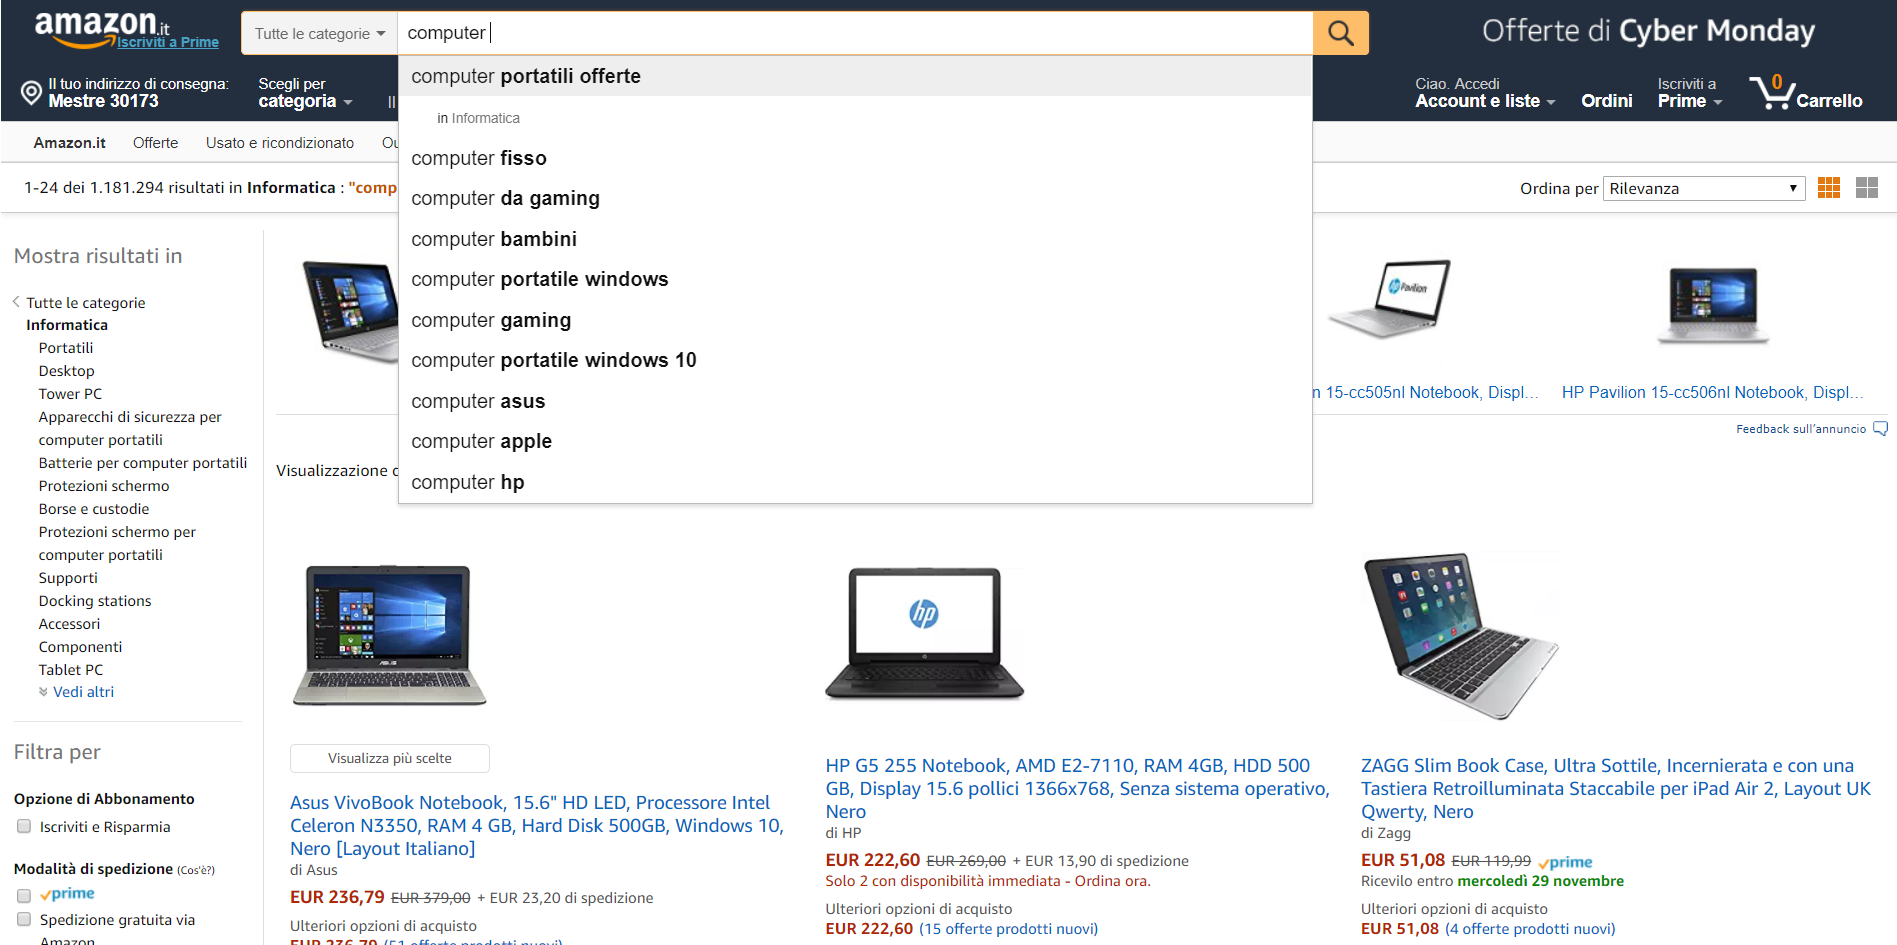
\includegraphics[width=13cm]{amazon}
			\captionof{figure}{Esempi di funzionalità di ricerca offerte dal sito di Amazon}
		\end{center}
	\end{figure}
	
	I motori di ricerca hanno assunto un ruolo fondamentale per gli utenti che navigano i siti web. Il genere di contatto che arriva da un motore di ricerca è particolarmente importante, in quanto quest'ultimo non rappresenta un utente passivo, bensì è un'entità attiva, pronta ad interagire con il suo utilizzatore. Durante una ricerca infatti, solitamente l'utente immette delle parole chiave, sperando di trovare ciò che sta cercando, con grandi aspettative derivanti dalla consultazione dei risultati. \\
	Per aiutare l'utente a trovare ciò che sta cercando, i siti web devono però fare la loro parte: è necessario infatti che vengano curati con particolare attenzione alla visibilità elementi come testi e parole chiave.\\
	Navigando i siti web, l'utente può trovare vari strumenti, messi a sua disposizione, che hanno lo scopo di aiutarlo a trovare quello che sta cercando. Tra i più importanti, troviamo:
	\begin{itemize}
		\item {\textbf{Menù}: rappresentano delle categorizzazioni delle pagine; è necessario che queste siano ben categorizzate e le voci dei menù devono essere chiaramente distinguibili l'una dall'altra. Inoltre, è fortemente sconsigliato un numero elevato di voci e di sottomenù: l'utente deve infatti poter ritrovare l'informazione che cerca in un numero molto limitato di click. Per siti che contengono una grande mole di informazioni, contenute in un gran numero di pagine, questo strumento risulta dunque essere utile ma non sufficiente, in quanto non rappresenta per l'utente uno strumento attraverso il quale trovare agevolmente i contenuti di interesse in un sito contenente una grande mole di documenti;}
		\item{\textbf{Search Box}: l’utente deve inserire in un campo di testo una o più parole chiave. Eventualmente, è possibile disporre di una ricerca avanzata, specificando uno o più filtri. Qualsiasi etichetta o filtro che permetta di inserire criteri come “cerca solo la parola esatta” oppure “escludi dalla ricerca le seguenti parole” funziona solamente se l’utente è capace di esprimere in termini logici i criteri che ha in mente. Per essere efficace, è dunque di fondamentale importanza disporre di una ricerca che sia il più possibile in grado di comprendere il linguaggio naturale dell'utente;}
		\item{\textbf{Faceted Search}: questo strumento estende l'idea dei semplici filtri di ricerca, consentendo di ricercare elementi attraverso filtri multipli, comprendendo quindi più attributi per volta nella ricerca.}
	\end{itemize}
	
	Lo scopo dello stage consisteva nell'analisi delle caratteristiche dei motori di ricerca \gls{open source} nell'ambito dei siti web di tipo informativo e, in particolare, lo studio e il confronto delle funzionalità di possibile interesse per i siti web istituzionali delle Camere di Commercio. L'obiettivo da raggiungere, consiste nel cercare di migliorare l'esperienza di navigazione, da parte degli utenti, all'interno dei siti camerali, rendendo la navigazione il più possibile efficiente, efficace e semplice. \\
	Per raggiungere questo obiettivo, in primo luogo mi è stato richiesto un approfondimento delle caratteristiche istituzionali dei siti web delle Camere di Commercio. \\
	Successivamente, l'azienda richiedeva lo studio della tecnologia \gls{Drupal} e dell'analisi delle potenzialità e specificità dei motori di ricerca \gls{Solr} e \gls{ElasticSearch}. \\
	Veniva inoltre richiesto un prototipo di un sito web in tecnologia \gls{Drupal}, con i due motori di ricerca precedentemente citati. \\
	Infine, era richiesta una relazione finale sulle potenzialità emerse nell'utilizzo dei due motori di ricerca. \\
	
	\subsection{Obiettivi posti dall'azienda}
	
		\subsubsection{Le milestone}
		Il Piano di Lavoro, redatto assieme al tutor aziendale che mi ha seguito durante lo stage in \nomeAzienda, prevede, tra l'altro, una serie di \gls{Milestone}; ad ognuna di esse, sono associati i prodotti sviluppati entro ogni corrispondente scadenza. Di seguito ne riporto l'elenco completo:
		
		\begin{itemize}
			\item {Fine prima settimana: Ambiente di sviluppo configurato e funzionante (n.b. per ambiente di sviluppo si intende installazione in locale di un sito web \gls{Drupal});}
			\item {Fine seconda settimana: Relazione con approfondimenti riguardanti \gls{Solr};}
			\item {Fine quarta settimana: Realizzazione prototipo di sito web in \gls{Drupal} integrato con \gls{Solr};}
			\item {Fine quinta settimana: Relazione con approfondimenti riguardanti \gls{ElasticSearch};}
			\item {Fine settima settimana: Realizzazione prototipo di sito web in \gls{Drupal} integrato con \gls{ElasticSearch};}
			\item {Fine ottava settimana: Relazione conclusiva e presentazione dell’elaborato al team di lavoro.}		
		\end{itemize}

		\begin{figure}[htbp]
			\begin{center}
				
\includegraphics[width=10cm]{milestone}
				\captionof{figure}{Milestone e metodologia di lavoro}
			\end{center}
		\end{figure}
	
		\subsubsection{Prodotti attesi}		
		L'attività di stage prevedeva la produzione di un insieme di oggetti, frutto di tale attività. Di seguito, ne è riportato l'elenco:
		
		\begin{itemize}
			\item {Documento: relazione sul motore di ricerca \gls{Solr} che riporti le caratteristiche funzionali ed architetturali della soluzione, pregi e difetti e possibile utilizzo all'interno del contesto InfoCamere;}
			\item {Documento: relazione sul motore di ricerca \gls{ElasticSearch} che riporti le caratteristiche funzionali ed architetturali della soluzione, pregi e difetti e possibile utilizzo all'interno del contesto InfoCamere;}
			\item {Documento: relazione finale di comparazione dei due motori di ricerca;}
			\item {Software: prototipo di sito web in tecnologia \gls{Drupal} che utilizza motore di ricerca \gls{Solr};}
			\item {Software: prototipo di sito web in tecnologia \gls{Drupal} che utilizza motore di ricerca \gls{ElasticSearch};}
			\item {Documento: relazione conclusiva (slide) sull'esperienza dell'uso dei prototipi, pregi e difetti nell'uso dei motori di ricerca in \gls{Drupal} e comparazioni}.
		\end{itemize}
	
		\subsubsection{Priorità degli obiettivi aziendali}
		Gli obiettivi aziendali riguardanti lo stage possono essere suddivisi in:
		\begin{itemize}
			 \item[--] {obiettivi minimi: vincolanti in quanto richieste primarie del committente;}
			 \item[--] {obiettivi massimi: non vincolanti o strettamente necessari, ma dal riconoscibile valore aggiunto.}
	 	\end{itemize}
 	
		Di seguito, vengono riportati gli obiettivi minimi e massimi stabiliti:
		
		\begin{longtable}{| C{2cm} | C{9cm} |}
			\toprule
			\textbf{ID} & \textbf{Descrizione} \\ \hline
			\endhead	% Permette di ripetere l'intestazione nelle nuove pagine
			\midrule
			
			%%%%%	INIZIO BLOCCO FUNZIONALITA'	%%%%%
			
			\multicolumn{2}{|c|}{\cellcolor[HTML]{EFEFEF}\textbf{Obiettivi obbligatori (min) }} \\ \hline
			
				%%%%%	INIZIO BLOCCO TEST	%%%%%
				
				min01 &  Analisi dei punti di forza e debolezza dei prodotti \gls{Solr} ed \gls{ElasticSearch} \\ \hline
				
				%%%%%	FINE BLOCCO TEST	%%%%%
				
				%%%%%	INIZIO BLOCCO TEST	%%%%%
				
				min02 &  Realizzazione del prototipo in \gls{Drupal} con le funzioni minime di ricerca  \\ \hline
				
				%%%%%	FINE BLOCCO TEST	%%%%%

			%%%%%	FINE BLOCCO FUNZIONALITA'	%%%%%



			%%%%%	INIZIO BLOCCO FUNZIONALITA'	%%%%%

			\multicolumn{2}{|c|}{\cellcolor[HTML]{EFEFEF}\textbf{Obiettivi desiderabili e opzionali (max) }} \\ \hline
			
				%%%%%	INIZIO BLOCCO TEST	%%%%%
				
				max01 & Comparazione dei due motori di ricerca esaminati con altri di riferimento nel mercato \\ \hline
				
				%%%%%	FINE BLOCCO TEST	%%%%%
				
				%%%%%	INIZIO BLOCCO TEST	%%%%%
				
				max02 &  Indicazioni su possibili interventi sui siti web istituzionali per quanto riguarda la user experience di navigazione, a seguito delle potenzialità espresse dai motori di ricerca   \\ \hline
				
				%%%%%	FINE BLOCCO TEST	%%%%%
			
			%%%%%	FINE BLOCCO FUNZIONALITA'	%%%%%
			
			\bottomrule
			\caption{Obiettivi dello stage}
		\end{longtable}
		

	\subsection{Vincoli}
	
	\begin{figure}[htbp]
		\begin{center}
			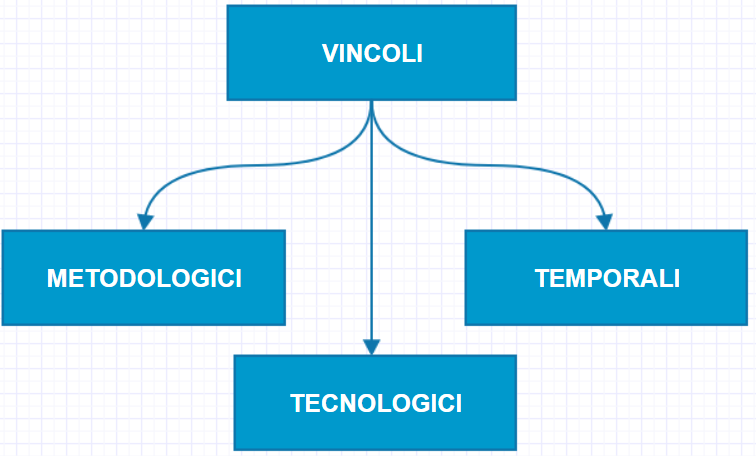
\includegraphics[height=6cm]{vincoli}
			\captionof{figure}{Tipologie di vincoli del progetto}
		\end{center}
	\end{figure}
	
		\subsubsection{Vincoli metodologici}
		In accordo con \nomeAzienda, ho svolto lo stage presso la sede di \locazioneAzienda. In questo modo, ho avuto la possibilità di confrontarmi con programmatori più esperti ed essere supportato al meglio in caso di problematiche di sviluppo e gestione del progetto; lo svolgimento dello stage in azienda aveva inoltre lo scopo di favorire l’inserimento dello stagista nell'area di sviluppo aziendale.
		Ho avuto la possibilità, a cadenza quotidiana, di discutere con il tutor aziendale per qualsiasi tipo di problema legato allo stage. Settimanalmente, abbiamo fatto il punto della situazione sullo stato del lavoro, rivedendo, quando necessario, obiettivi settimanali o eventuali miglioramenti al progetto. \\
		Nell'ultima settimana lavorativa, l'azienda ha inoltre richiesto una presentazione, esposta verbalmente e corredata da diapositive illustrative, sul lavoro operato durante lo stage e sulle relative conclusioni. \\
		Altro vincolo legato alla metodologia, riguarda invece la tipologia di installazione dell'ambiente di sviluppo. In accordo con il tutor aziendale, ho deciso di installare l'intero ambiente di sviluppo localmente, così da poter intervenire agevolmente sull'intero sistema, senza la necessità di coinvolgere i sistemisti (o comunque altri reparti aziendali), per apportare modifiche a configurazioni delle tecnologie utilizzate, in modo tale da velocizzare i tempi di intervento.
		
		\subsubsection{Vincoli tecnologici}
		Per la gestione di versione dei prodotti dello stage, InfoCamere mi ha predisposto un repository \gls{Git}, nel quale ho versionato le varie istanze dei siti \gls{Drupal} creati, assieme ai relativi \gls{Dump} dei database, oltre ai documenti scritti. \\
		Per quanto concerne la tecnologia di comunicazione, mi sono invece state fornite delle credenziali di accesso, per poter accedere all'intranet aziendale e al client di posta elettronica utilizzato da \nomeAzienda (\gls{Zimbra}), oltre a consentirmi l'accesso all'account del PC della postazione che mi è stata assegnata. \\
		Per la presentazione finale fatta in azienda ho invece utilizzato un template aziendale dedicato alle presentazioni, realizzato con Microsoft PowerPoint. \\
		Infine, le istanze \gls{Drupal} create su \gls{Acquia Dev Desktop 2} sono state realizzate in locale, seppur questa tecnologia fornisca la possibilità di ospitare le istanze sulla piattaforma \gls{Acquia Cloud}. Così facendo, è possibile non dipendere in alcun modo da tempistiche legate alla tipologia di un eventuale account su \gls{Acquia Cloud}. In futuro, sarà dunque possibile per l'azienda disporre liberamente delle istanze da me create.
		
		\subsubsection{Vincoli temporali}
		L'orario di lavoro era lo stesso previsto per il personale \nomeAzienda: dal Lunedì al Venerdì, con orari flessibili di un'ora dalle 08.00-09.00 alle 17.00-18.00 con un'ora di pausa pranzo. \\
		L'azienda mi ha fornito un badge per accedere ai locali aziendali e mi è stato inoltre richiesto di timbrare quotidianamente il badge per registrare gli orari di entrata e di uscita. Inoltre, a cadenza quotidiana, il tutor aziendale registrava le attività svolte, la data e apponeva infine la propria firma. \\
		Il numero complessivo di ore previsto dallo stage era pari a circa 300 ore, distribuite nell'arco di due mesi, con settimane lavorative di 40 ore ciascuna.

\section{Obiettivi personali}
Personalmente, ritengo che svolgere uno stage sia molto importante nell'odierno mercato del lavoro; questa opportunità porta infatti benefici, oltre che all'azienda, allo stagista stesso, sia dal punto di vista personale, sia da quello professionale. \\
Uno studente universitario apprende, nel corso del proprio percorso formativo scolastico, un gran numero di nozioni teoriche. Allo stesso tempo però, gli studenti hanno carenze sull'aspetto pratico del lavoro. Per poter sopperire a queste mancanze, permettendo allo studente di essere più competitivo nel mercato del lavoro, è di fondamentale importanza arricchire le conoscenze teoriche con esperienze professionali. \\
Lo stage permette allo studente di fare esperienza senza la necessità, da parte dell'azienda, di assumere personale privo di esperienza. \\
Oltre alle sopraccitate motivazioni, riporterò di seguito i motivi che mi hanno portato a scegliere, tra le tante aziende con le quali sono venuto a contatto grazie all'evento StageIT, \nomeAzienda.

\begin{itemize}
	\item {Motivazioni professionali: Essendo stata questa la mia prima esperienza lavorativa in un'azienda che lavora in ambito informatico, ho scelto \nomeAzienda, azienda con un gran numero di dipendenti e particolarmente strutturata, con la speranza di potermi confrontare con gente molto più esperta di me, con conoscenze più specifiche e capacità di problem solving differenti rispetto a quelle che si possono trovare nel mondo universitario. Inoltre, ho ritenuto l'argomento dello stage di particolare interesse, in grado di fornirmi abilità molto richieste nell'attuale mondo del lavoro. Oltre a tutto questo, ritengo inoltre di fondamentale importanza ampliare la mia rete di contatti con professionisti che lavorino nel mio stesso campo d'interesse, utile per eventuali consigli professionali, raccomandazioni di lavoro, o più semplicemente per avere confronti costruttivi. Infine, l'esperienza porterà certamente ad un valore aggiunto al mio curriculum.
}
	
	\item {Motivazioni economiche: A differenza di altre aziende con cui ho avuto un contatto, \nomeAzienda offriva un rimborso spese e buoni pasto. Ritengo che questo tipo di riconoscimento da parte dell'azienda sia un modo per incentivare lo stagista a svolgere al meglio il proprio lavoro, oltre ad agevolare lo studente, aiutandolo a sostenere le spese che deve sostenere.}
	
	\item {Motivazioni personali: Ritengo che lo stage sia il momento adatto per capire se il lavoro che ho scelto e la strada che ho intrapreso sia realmente ciò che voglio fare nella mia vita.}
	
\end{itemize}


%Senza ombra di dubbio c'è appunto la possibilità di apprendere  un mestiere e conoscerne quindi pregi e difetti prima di entrare in azienda come dipendente. Lo stage è anche un ottimo momento dove potersi "schiarire le idee" e capire quindi se il vostro percorso di studi, legato alla vostra futura professione, è certamente quello che vorrete fare nella vostra vita. 